% Number 961
% CAPMA CVPMA Algebra Units 
% Drag racer - CAPM and CVPM - algebraic
% JG

% Watermark
\AddToShipoutPicture*{\BackgroundPic}

\addtocounter {ProbNum} {1}

%\begin{floatingfigure}[r]{.44\textwidth}
%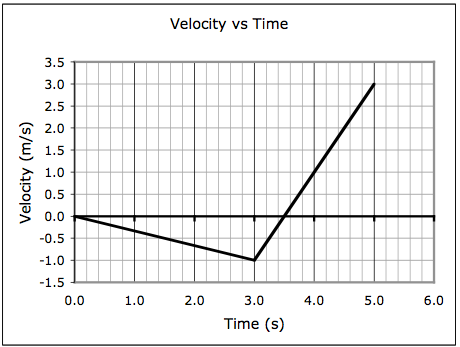
\includegraphics[scale=.54]{/Users/jgates/desktop/latex/pics/vgraph6}
%\end{floatingfigure}
 
{\bf \Large{\arabic{ProbNum}}} A drag racer begins at rest, and accelerates to ${124~\tfrac{m}{s}}$ within 2.2 seconds.  Once at this speed, the racer maintains it through the finish line, which is 400 meters from the start line. \bigskip

How long does it take for the driver to finish the race?
\vfill

The car deploys a parachute after crossing the finish line.  The magnitude of the acceleration provided by the air hitting the parachute is ${12~\tfrac{m}{s^2}}$.  How far will the car travel while the parachute is stopping it? 

\vfill

What assumptions did you make to solve this problem?  Are they good assumptions?
\vspace{30mm}
%\begin{center}
%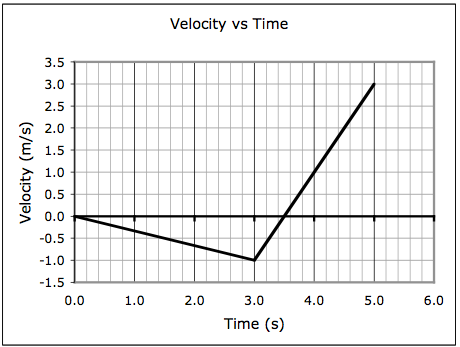
\includegraphics[scale=1]{/Users/jgates/desktop/latex/pics/vgraph6}
%\end{center}


\newpage